% =====================================================================
%  Airway segmentation and anatomical branch assignment in pediatric CT
%  LNCS / MICCAI format. Submission version.
%
%  The long working document, which carries the full derivations, every
%  table and all open questions, is airway_method_paper_FULL_working.tex.
%  Detail belongs there, or in a supplement if one is submitted, not here.
%
%  Style rules: no em dashes, no semicolons in body prose.
%  Compile: tectonic -X compile airway_method_paper.tex
% =====================================================================
\documentclass[runningheads]{llncs}

\usepackage{graphicx}
\usepackage{booktabs}
\usepackage{array}
\usepackage{makecell}
\usepackage{amsmath}
\usepackage{amssymb}
\usepackage{xcolor}
\usepackage[hidelinks]{hyperref}
\usepackage{tikz}
\usetikzlibrary{arrows.meta,positioning,fit,backgrounds,calc}
\renewcommand\UrlFont{\color{blue}\rmfamily}

% A small stretch allowance keeps the narrow LNCS measure from overflowing
% rather than forcing awkward rewrites of otherwise correct sentences.
\setlength{\emergencystretch}{1em}

\newcommand{\todo}[1]{\textcolor{gray}{\textit{[#1]}}}

% Block diagram styles. Fills are light so that the labels stay legible after
% the page reduction, and the two stages of the pipeline are separated by fill
% rather than by a box, which would cost vertical space.
\definecolor{segfill}{HTML}{DCE9F7}
\definecolor{segline}{HTML}{2A78D6}
\definecolor{labfill}{HTML}{E6E0F5}
\definecolor{labline}{HTML}{6B4FBB}
\definecolor{iofill}{HTML}{ECECE8}
\tikzset{
  blk/.style={draw, rounded corners=2pt, align=center, inner sep=3.2pt,
              font=\scriptsize, minimum height=7.5mm, line width=0.5pt},
  seg/.style={blk, fill=segfill, draw=segline},
  lab/.style={blk, fill=labfill, draw=labline},
  io/.style={blk, fill=iofill, draw=black!55},
  op/.style={draw, circle, inner sep=0.8pt, font=\scriptsize, line width=0.5pt,
             fill=segfill, draw=segline},
  fl/.style={-{Latex[length=1.6mm,width=1.4mm]}, line width=0.5pt, draw=black!70},
  note/.style={font=\tiny, text=black!60, align=center},
}
\newcommand{\hd}[1]{\makecell[c]{#1}}

\begin{document}

\title{Airway Segmentation and Anatomical Branch Assignment\\in Pediatric Chest CT}
\titlerunning{Pediatric airway segmentation and branch assignment}

% ANONYMOUS FOR REVIEW. The real block is kept below so it can be restored in
% one edit. The marker meanings are assumed and need confirming: star for equal
% first authorship, double star for equal senior authorship, dagger for the
% corresponding author.
%
% \author{%
% Huseyin Umut Isik\inst{1}\textsuperscript{$\star$} \and
% Ege Mert Balcik\inst{1}\textsuperscript{$\star,\dagger$} \and
% Sila Kurugol\inst{3}\textsuperscript{$\star\star$} \and
% \c{S}eyda Ertekin\inst{1,2}\textsuperscript{$\star\star$}}
% \authorrunning{H. U. Isik et al.}
% \institute{Department of Computer Engineering, METU, Ankara, Turkey \and
% METU-DTX Digital Transformation and Innovation Center, Ankara, Turkey \and
% Quantitative Intelligent Imaging Lab, Boston Children's Hospital and Harvard
% Medical School, Boston, MA, USA}
%
% Restoring the block above also means restoring the marker footnote that used
% to follow \maketitle, and the acknowledgement and funding text.
\author{Anonymous}
\authorrunning{Anonymous}
\institute{Paper submitted for blind review}

\maketitle

\begin{abstract}
A segmented airway tree answers few clinical questions until its branches are
named, and the methods that segment airways and the recent work that names them
are developed and validated almost entirely in adults. For an automated method
the pediatric airway is not a smaller version of the adult one. Branch calibre
approaches the voxel size, one model has to cover the range of physical sizes
between a newborn and an adolescent, and acquisition is lower dose and often
without breath hold. These differences change how a method fails rather than
only how well it scores. We combine three public airway models by union and
retain a single connected component chosen by a seed rather than by size, then
name every branch with a graph transformer that had to be trained here because
its weights were never released. Evaluation covers a public adult benchmark,
public branch-wise anatomical labels, and nine expert-annotated volumes from a
balanced pediatric cohort spanning birth to adolescence. Combining models is
worth far more in children than in adults. It raises the percentage of reference
branches detected by 6.0 points over the best pair of models, where the same
gain on the adult benchmark is 0.7. Retaining
the largest connected component instead of the seeded one destroys the airway
silently, and every pediatric examination where it does so is an infant under
one year. Segmentation accuracy falls steeply with depth while naming accuracy
stays near flat, so branch recovery rather than naming is what limits the
pipeline. The method is released as a fully automated open web application:
a de-identified CT is uploaded and the segmented, named and measured airway
tree comes back in an in-browser 3D viewer, with no installation and no local
GPU. With it we release an extension of ITK-SNAP that edits a segmentation
directly in the 3D view, so that the peripheral defects an automatic airway
segmentation leaves can be corrected where they are seen.

\keywords{Airway segmentation \and Anatomical labelling \and Pediatric chest CT
\and Model ensemble \and Web application \and ITK-SNAP.}
\end{abstract}

% =====================================================================
\section{Introduction}
\label{sec:intro}

Most questions asked of an airway tree are asked about a particular branch. A
bronchoscopist needs the segmental bronchus that leads to a lesion, a
radiologist reporting bronchiectasis needs the affected lobe and segment, and a
morphometric study needs the same anatomical branch across subjects. A binary
mask supports none of these on its own. Anatomical labelling is therefore a second task on top of
segmentation, and recent work addresses it at lobar, segmental and subsegmental
resolution \cite{zhang2025airmorph}.

That work, and the segmentation methods it builds on \cite{carmo2024medpseg,wu2025tfenet}, was developed and validated in adults. The pediatric airway
differs in ways that matter for an automated method. Calibre relative to voxel
size is smaller, so a mid-generation bronchus in an infant may span only a few
voxels and the partial-volume boundary becomes a large fraction of the
structure. One model must cover a range of physical sizes an adult model never
sees, and acquisition is lower dose and often without breath hold.

These differences change how a method fails rather than only how well it scores.
A permissive network produces spurious structures, and in a small airway such a
structure can exceed the true tree in volume, at which point the routine step of
retaining the largest connected component discards the airway and keeps the
artefact. The failure is silent, because the retained object still resembles an
airway tree, and whole-tree accuracy conceals it because the proximal
generations carry most of the voxels while the peripheral generations are
exactly those most affected by resolution.

\smallskip\noindent\textbf{Contributions.}
(i) A branch assignment stage for the pediatric airway tree, following the
architecture of \cite{zhang2025airmorph}, whose weights were never released and
whose description is incomplete, so the training procedure was reconstructed
here with every open choice stated explicitly. (ii) An ensemble segmentation
front end with a seeded component-selection rule that removes the silent failure
above. (iii) A generation-limited evaluation protocol for settings where an
exhaustive expert reference is unattainable. (iv) A pediatric benchmark of the
segmentation front end on nine expert-annotated volumes, with the bias its
annotation provenance introduces measured and stated. (v) An open-source web
application that runs the complete pipeline on an uploaded de-identified CT and
returns the mask, the named tree, an in-browser viewer and per-branch
morphometry, so that the method can be used from a browser without any local
installation. (vi) An extension of ITK-SNAP that edits a segmentation directly
in the 3D view, written to correct airway trees whose defects are visible only
in 3D. (vii) A calibrated confidence for every voxel and every branch of the
fused mask, read off the ensemble's vote pattern without retraining, which
places 86 per cent of the false-positive voxels in the least confident fifth
of the mask and, used to trim the mask, raises adult DSC by one point at
a cost of one point of branch detection. We make no claim of superiority over state-of-the-art segmentation
models and report no such comparison.

% =====================================================================
\section{Data}
\label{sec:data}

\textbf{Public benchmark.} The binary airway segmentation task of the Airway
Tree Modeling challenge \cite{atm22} provides 299 annotated thoracic CT
volumes, partitioned
once with a fixed seed into 239 training, 30 validation and 30 test volumes.
Every benchmark value below is computed on the 30 test volumes, which were
withheld from all development.

\textbf{Anatomical labels.} A second annotation set covers 118 of those volumes
with branch-wise anatomical labels. The 11 that also fall in the segmentation
test set were reserved as the labelling test split and the remaining 107
supplied labelling training and validation, so no volume used to evaluate
labelling contributed to training either stage.

\textbf{Pediatric cohort.} Ninety examinations from 90 distinct patients aged
0.2 to 18.0 years, drawn by integer programming from two processed cohorts, with
exactly ten examinations in each of nine two-year age bands, at most one scan per
patient, and sex recorded for all. The cohort is 43 male and 47 female. Where a
result is reported on the larger screened pool rather than the balanced cohort,
83 examinations, this is stated. Nine of these examinations carry an expert
airway annotation, drawn by three annotators.
\todo{IRB approval, consent, de-identification.}

% =====================================================================
\section{Method}
\label{sec:method}

\begin{figure}[tbp]
\centering
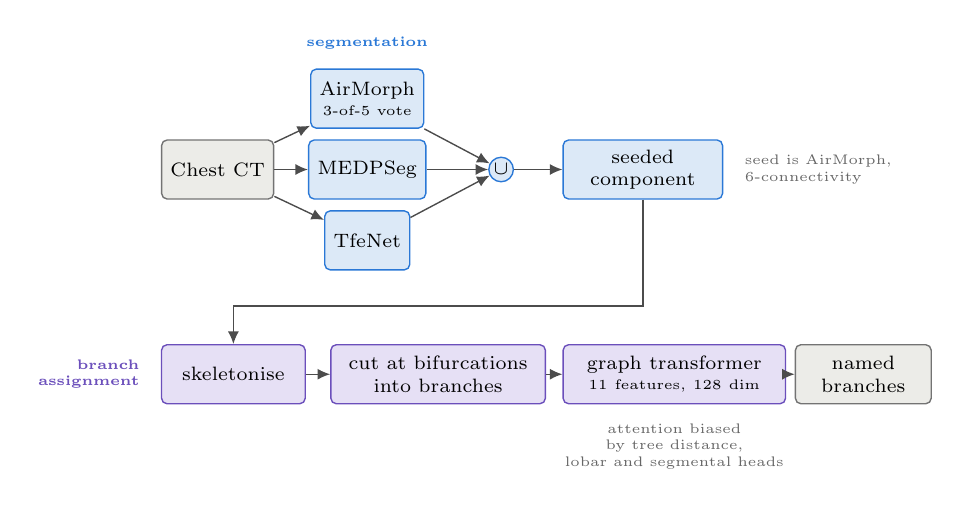
\begin{tikzpicture}

% ---- row 1, the segmentation front end
\node[io] (ct) {Chest CT};
\node[seg] (mp) at ($(ct)+(19mm,0)$) {MEDPSeg};
\node[seg] (am) at ($(mp)+(0,9mm)$) {AirMorph\\[-1pt]\tiny 3-of-5 vote};
\node[seg] (tf) at ($(mp)+(0,-9mm)$) {TfeNet};
\node[op]  (or) at ($(mp)+(17mm,0)$) {$\cup$};
\node[seg, text width=18mm] (lcc) at ($(or)+(18mm,0)$) {seeded\\component};
\node[note, right=1.5mm of lcc, text width=21mm, align=left]
  {seed is AirMorph,\\6-connectivity};
\draw[fl] (ct) -- (am); \draw[fl] (ct) -- (mp); \draw[fl] (ct) -- (tf);
\draw[fl] (am) -- (or); \draw[fl] (mp) -- (or); \draw[fl] (tf) -- (or);
\draw[fl] (or) -- (lcc);

% ---- row 2, branch assignment. The connector runs in a clear channel between
% the rows, so it crosses no block.
\node[lab, text width=16mm] (sk) at ($(ct)+(2mm,-26mm)$) {skeletonise};
\node[lab, text width=25mm] (pc) at ($(sk)+(26mm,0)$) {cut at bifurcations\\into branches};
\node[lab, text width=26mm] (gt) at ($(pc)+(30mm,0)$)
  {graph transformer\\[-1pt]\tiny 11 features, 128 dim};
\node[io, text width=15mm] (out) at ($(gt)+(24mm,0)$) {named\\branches};
\draw[fl] (sk) -- (pc); \draw[fl] (pc) -- (gt); \draw[fl] (gt) -- (out);
\node[note, below=1.2mm of gt, text width=32mm]
  {attention biased by tree distance,\\lobar and segmental heads};

\coordinate (ch) at ($(lcc.south)+(0,-13.5mm)$);
\draw[fl] (lcc.south) -- (ch) -| (sk.north);

% ---- which stage is which
\node[note, above=1.2mm of am, text width=30mm, text=segline]
  {\textbf{segmentation}};
\node[note, left=1.5mm of sk, text width=13mm, align=right, text=labline]
  {\textbf{branch\\assignment}};
\end{tikzpicture}
\caption{The pipeline as blocks. One chest CT is segmented independently by
three public models, their masks are combined by a bitwise union, and a single
connected component is retained by seeding it from the AirMorph mask rather than
by taking the largest one. That mask is skeletonised, the skeleton is cut at
bifurcations into branches, and a graph transformer names each branch from its
geometry and its position in the tree. Figure~\ref{fig:pipeline} shows the same
stages as images on one examination.}
\label{fig:arch}
\end{figure}

\begin{figure}[tbp]
\centering
\includegraphics[width=\textwidth]{figures/03_pipeline.pdf}
\caption{The pipeline on one examination, the 0.9-year-old infant used
throughout. \textbf{(a) Computed tomography}, as a minimum intensity projection
through the same slab as the renders beside it, so that the airway lumen reads
as a dark tree against aerated lung. \textbf{(b) Airway segmentation}, the
three-model union under seeded component selection. \textbf{(c) Centreline}.
\textbf{(d) Branch parcellation}, the centreline cut at bifurcations into 164
branches, each in its own colour, which are the nodes the graph transformer
receives. \textbf{(e) Anatomical assignment}, the predicted label of every
branch painted back onto the airway surface. Branches proximal to the lobar
division carry the tracheal class, which is how the annotation vocabulary treats
them. Panels (b) to (e) share one crop, camera and light, so only the
representation changes.}
\label{fig:pipeline}
\end{figure}

\subsection{Segmentation}
Figure~\ref{fig:pipeline} shows the whole pipeline on one examination. Three
airway models are run independently and their binary masks combined by a bitwise
OR. Component pruning is applied once, to the union, rather than to each member,
because a detached distal fragment from one member is precisely what another
member's mask is meant to reconnect. The retained component is the one
containing the most voxels of a designated seed member, under
6-connectivity.\footnote{Common libraries encode this as
\texttt{connectivity}~$=1$, where 2 and 3 denote the 18- and 26-neighbourhood.}
Selecting by size instead fails when a member emits a component larger than the
airway and disjoint from it, which is the failure quantified in
Section~\ref{sec:res-selection}. If the seed does not intersect the union the
rule falls back to the largest component.

Figure~\ref{fig:panels} shows the stage in detail. Two members are released
checkpoints \cite{carmo2024medpseg,wu2025tfenet} and the seed is a
three-of-five vote of architectures trained on the 239-volume split. Source volumes are LAS and two of the three models ignore direction
cosines, so reorientation is applied in both directions and verified
quantitatively by sampling the original CT at the final mask voxels, which must
return air density.

\subsection{Confidence map and uncertainty-aware refinement}
\label{sec:confidence}
Figure~\ref{fig:unc-arch} places the stage in the pipeline. A union keeps
whatever any one member marks, so part of the mask rests on a
single model, and the mask itself does not say which part. The seven
predictors behind it, AirMorph's five member networks (its mask is their
three-of-five vote), MEDPSeg and TfeNet, mark each fused voxel in one of 24
\emph{vote patterns}. On the 30 validation volumes we count, per pattern, the
fraction of voxels that are reference airway. That table is the confidence
map: $P(\text{airway}\mid\text{pattern})$ for every voxel, with no training and
no change to the members. A branch's confidence is the mean of the map along
its centreline, and the web application shows both (Section~\ref{sec:tools}).
The table is informative in itself. AirMorph's internal agreement is weak
evidence on its own, a 5-of-5 vote with neither other model is 53 per cent
airway and a 3-of-5 vote 17 per cent, whereas MEDPSeg and TfeNet agreeing
without AirMorph is 98 per cent airway. It is agreement \emph{between} models
that carries the information.

The map also allows the mask to be tidied without giving up the completeness
the union was adopted for. The fused mask is skeletonised and cut into
branches, every voxel is assigned to its nearest branch, and a voxel is kept
when its confidence is at least a fraction $\kappa$ of the confidence along
its branch's centreline; the core within $\max(0.5\,r, 1.5\text{ voxels})$ of
the centreline is always kept and the seeded-component rule is applied once
more. A branch all three models see is trimmed towards their consensus; a
distal branch that one model found keeps every voxel, because nothing in it
has more support than its own centreline. The branch tree also admits
topology-preserving pruning of improbable leaves, scored by a logistic
regression on branch evidence and geometry fitted on the validation
branches; it removed false branches but changed no metric measurably, and
is off by default. $\kappa$ was chosen on validation as the largest DSC gain
with at most one point of branch-detection loss, giving $\kappa=0.4$.

\begin{figure}[tbp]
\centering
\includegraphics[width=\textwidth]{figures/08_architecture_uncertainty.pdf}
\caption{The uncertainty-aware ensemble. The segmentation front end of
Figure~\ref{fig:arch} is unchanged; the seven predictors behind it mark every
fused voxel with one of 24 vote patterns, the pattern's precision on the
validation split is the voxel's confidence, and the confidence is shown as it
is, summarised per branch, and optionally used to trim each branch's boundary
relative to the confidence of its own centreline.}
\label{fig:unc-arch}
\end{figure}

\subsection{Branch assignment}
The fused mask is skeletonised, the skeleton is cut into segments at bifurcation
voxels, every lumen voxel is assigned to its nearest segment, and a
parent-child tree is built. Generation is depth from the root plus one, so the
trachea is generation 1. Other conventions number differently.

Each segment becomes a graph node carrying 11 geometric features, and a graph
transformer with 128 hidden dimensions predicts a lobar, a segmental and a
subsegmental label per node, with attention biased by tree distance
\cite{zhang2025airmorph}. The weights were not released, so the network was
trained here and the choices the published description leaves open are stated
explicitly. The optimiser follows the published Adam at $5\times10^{-4}$. No
labelling loss is given, and cross-entropy with deep supervision over the heads
was adopted. The stated 32 attention heads contradict the released configuration
of four heads of dimension 32, and the configuration was followed so the trained
weights load into the released inference path unchanged. Training ran 600 epochs
with validation every 10, one graph per step, and the exported checkpoint is the
best validation epoch by the surrogate accuracy described next, 559 of 600. The
run took three hours and seven minutes on one GPU.

Of the 6 lobar, 20 segmental and 82 subsegmental heads only the first two are
supervised by real labels. The public annotations are a 20-value segmental
scheme, verified at the data, and no subsegmental reference was released, so the
subsegmental head was trained toward the base subsegment of each segment. Its
accuracy is therefore segment granularity expressed in subsegmental identifiers
and is not a subsegmental result, and we report lobar and segmental accuracy
only. This differs from \cite{zhang2025airmorph}, whose 127 subsegmental classes
come from a private annotation set. The inference path offers no abstention, so
a non-root branch predicted as tracheal at every level is flagged rather than
reported as anatomy.

\subsection{Evaluation}
Metric definitions differ between publications and are stated as implemented.
With $P$ the predicted and $G$ the reference airway voxels, DSC is
$2|P\cap G|/(|P|+|G|)$, precision $|P\cap G|/|P|$ and sensitivity
$|P\cap G|/|G|$. Tree length detected (TLD) is $|S_G \cap P|/|S_G|$ on the
reference centerline $S_G$, and clDice \cite{cldice} is the harmonic mean of
$|S_P\cap G|/|S_P|$ and $|S_G\cap P|/|S_G|$. A branch is detected (BND) when at
least 80 per cent of its reference centerline voxels lie inside $P$. TLD and BND
are voxel-count fractions with no spacing weighting, so a subsegmental
centerline voxel counts as much as a tracheal one. For per-generation
evaluation every reference voxel inherits the generation of its branch and
metrics are recomputed with the reference restricted to one generation, the
prediction left unrestricted, and predicted voxels attributed by the same
nearest-branch map. Pooling all generations reproduces the whole-tree values on
every case.


\begin{figure}[tbp]
\centering
\includegraphics[width=\textwidth]{figures/01_member_panels.pdf}
\caption{The segmentation stage on one examination, an infant of 0.9 years
whose airway carries an expert annotation of 3.8\,mL. Every panel shares one
crop, camera and physical scale, so what differs is the mask alone, and the
frame is set by the union so that nothing any member produced is cropped
away. Under each panel is the mask's Dice against the annotation. AirMorph
(a) is conservative and clean at 2.5\,mL, MEDPSeg (b) adds detached debris
to 11.6\,mL, and TfeNet (c) contributes two slab artefacts that bring it to
29.5\,mL, an order of magnitude above the airway, so its Dice is 16.8
although it covers more of the annotated tree than either other member.
Their union (d) inherits all of it, at 36.3\,mL and
Dice 14.9. Selecting the component carrying the seed rather than the
largest one recovers the airway (e), 2.7\,mL at Dice 88.3, the highest of every panel
and above the same rule applied to any member on its own (f to i). On this
examination the largest component is a slab, so the conventional rule would
have discarded the tree entirely. Panel (e) is rendered on a finer grid with
smoothing artefacts suppressed, which does not affect the Dice printed on
the panels, measured on the masks themselves.}
\label{fig:panels}
\end{figure}

\subsection{Deployment and correction tools}
\label{sec:tools}
Two tools make the pipeline usable outside this study, and both are released
with the code.\footnote{\url{https://github.com/quin-med-harvard-edu/airway-seg-and-labelling}}

The \emph{web application} runs the pipeline as described, unchanged, on a CT
uploaded as a de-identified NIfTI volume. The three members, the union, the
seeded component selection, the skeletonisation and the branch assignment run
as separate stages on one 24\,GB GPU, about ten minutes for a
$512\times512\times800$ scan, and the page reports progress stage by stage.
The result opens in a viewer laid out like ITK-SNAP, three orthogonal slices
and a 3D pane sharing one crosshair, with the airway, lobar, segmental and
per-branch labels and the confidence map of Section~\ref{sec:confidence} as
switchable overlays, the airway surface in 3D coloured by whichever is
selected, the branch under the cursor named in a readout, and each branch's
confidence beside its measurements, so that a reader sees which part of the
tree rests on one model alone. Below the viewer the tree is measured: length, inscribed and
cross-sectional diameter, branching angle and generation for every branch,
the central airways and their ratios, and per-generation and per-lobe
summaries. Given the patient's age, every measurement is also reported as a
percentile against the 90-examination cohort of Section~\ref{sec:data}. A
set of checks on the result is shown with it, such as a trachea that does not
reach the lung apex, a lobe to which no branch was assigned, or a tree far
sparser than the cohort, so that a reader is told what to distrust. Every
volume, the ITK-SNAP label descriptions and the measurements can be
downloaded, including a bundle that opens directly on the original CT in
ITK-SNAP. The service runs on
serverless GPU capacity that exists only while a scan is being processed, so a
lab without a GPU machine can offer it at a cost of cents per scan. It is
restricted to research use and to de-identified data, and says so on every
page.

The \emph{3D editing extension} addresses the correction step that any
automatic airway segmentation eventually needs. ITK-SNAP paints a
segmentation slice by slice and renders it as a surface, so a defect that is
obvious in 3D, a floating fragment, a leak into the parenchyma, a hole in the
lumen or a branch broken off from the tree, has to be found again in 2D before
it can be fixed. Our fork\footnote{\url{https://github.com/quin-med-harvard-edu/itksnap-3d-edit}}
adds an editing tool to the 3D view with four operations: a surface brush that
paints and erases on the rendered mesh, deletion of a disconnected component
in one click, a bridge that joins two structures with a tube, and a local
morphological closing that fills a hole. The brush picks its target on the
rendered isosurface rather than on the label image, so it can add material and
bridge gaps, which the existing 3D tools of ITK-SNAP cannot. Each stroke is
one undo step, the mesh refreshes after every edit, and deleting a large
component asks for confirmation. Nothing in it is specific to airways, but it
was built on pediatric airway trees, where the defects that matter are
peripheral and small and exactly the ones a 2D pass misses.

% =====================================================================
\section{Results}
\label{sec:results}

\subsection{Combination strategy}
Table~\ref{tab:variants} reports each model alone and every combination of them
on the benchmark test set. The two families of metric do not agree. Majority
voting attains the highest DSC, precision and surface distance, while the union
of all three members attains the highest TLD, BND and sensitivity. Every
combination sits between 1.43 and 1.82 mm of surface distance, under two voxels,
and the difference between the union and the best of them is not significant. We adopt the union,
because completeness governs whether a branch can be labelled at all, whereas a
branch recovered with a slightly inaccurate boundary can still be named.

The three models differ sharply in character. MEDPSeg is conservative and
accurate, at DSC 93.29 and precision 92.02, but detects only 76.10 per cent of
branches. TfeNet sits at the other extreme, at precision 53.68 and DSC 65.23,
and is no more complete for being permissive, reaching BND 75.65 against
MEDPSeg's 76.10. It still contributes, because what it adds is not what the
other two already hold. AirMorph is the strongest single model on topology at
BND 91.27 and the union improves on it by a full point. Within AirMorph one
member reaches TLD 95.40 alone, above the union's 95.22, while the union leads
on branch detection at 92.31 against that member's 91.68.

Whether that trade can be avoided was tested before settling on the union.
Fifty-one combination rules were scored on the 30 validation volumes, and none
dominated the union across all six metrics on either split. One rule does lead
four columns on test, but by admitting almost everything, at DSC 77.07 and
precision 63.53 against the union's 93.06 and 88.71. Completeness and boundary
agreement trade against each other here, and we take the completeness side
because that is what the next stage depends on.

\begin{table}[tbp]
\centering
\caption{Each model alone and every combination of them, on the 30 held-out
benchmark volumes. Component selection is the seeded rule throughout, and the
individual models are scored as the combination consumes them, before their own
post-processing. Majority vote is a voxel-wise two-of-three vote of the raw
masks, and ``selected'' applies the seeded component selection to it. The
strategy adopted for the rest of the paper is the union of all three members,
for the reason given in the text. HD95 is the 95th
percentile of the surface distance in millimetres, which the plain Hausdorff
distance cannot replace here because a single voxel sets it. Best value per
column in bold, second best underlined.}
\label{tab:variants}
\setlength{\tabcolsep}{3.5pt}\footnotesize
\begin{tabular}{@{}lccccccc@{}}
\toprule
Strategy & DSC & clDice & TLD & BND & Sens. & Prec. & \hd{HD95\\(mm)} \\
\midrule
AirMorph & 91.64 & 89.05 & \underline{94.95} & 91.27 & 95.04 & 89.12 & 2.77 \\
MEDPSeg & 93.29 & 85.82 & 87.50 & 76.10 & 94.78 & 92.02 & 2.36 \\
TfeNet & 65.23 & 51.03 & 86.54 & 75.65 & 91.44 & 53.68 & 133.70 \\
\midrule
AirMorph $\cup$ MEDPSeg & 93.15 & 90.32 & 94.44 & 91.29 & \underline{98.06} & 88.99 & 1.66 \\
AirMorph $\cup$ TfeNet & 93.29 & \textbf{90.81} & 94.80 & \underline{91.61} & 97.43 & 89.83 & 1.75 \\
MEDPSeg $\cup$ TfeNet & \underline{94.08} & 90.06 & 88.96 & 81.91 & 95.96 & 92.55 & \underline{1.64} \\
All three members & 93.06 & 90.24 & \textbf{95.22} & \textbf{92.31} & \textbf{98.23} & 88.71 & 1.81 \\
\midrule
Majority vote & 94.04 & 89.63 & 90.94 & 83.19 & 95.51 & \underline{93.07} & 1.82 \\
Majority vote, selected & \textbf{94.38} & \underline{90.48} & 87.84 & 80.35 & 95.00 & \textbf{94.04} & \textbf{1.43} \\
\bottomrule
\end{tabular}
\end{table}

\subsection{Component selection}
\label{sec:res-selection}
Replacing the seeded rule with largest-component selection affected three of the
four union strategies, each on the same three examinations, where the retained
mask had no overlap at all with the reference and every metric scored zero.
Across the four unions this is 9 of 120 pairs, with the same component retained
on the remaining 111, and the union without the permissive member was never
affected, consistent with the mechanism. On the three affected examinations the
retained component measured 242\,471, 126\,664 and 128\,539 voxels against the
true airway's 198\,567, 122\,161 and 97\,738. At test-set level the effect is a
change in dispersion rather than a uniform loss. Mean DSC for the union of all
three falls from 93.06 to 84.57 while the standard deviation rises from 4.37 to
28.74, so the distribution is bimodal rather than degraded.

In children the rule matters far more. Across 83 screened pediatric
examinations the two rules disagreed on six, and every one was an infant under
one year of age, six of the nine such examinations present, while they agreed on
all 74 aged one year and above. The comparable adult figure is three of 30.

\subsection{Accuracy by generation}
Table~\ref{tab:gen} and Figure~\ref{fig:gen} report accuracy generation by
generation, for the adopted union and for each member alone. For the union the
whole-tree DSC of 93.06 describes no generation well, falling from 98.39 at the
trachea to 74.73 at generation 10 and dropping below 90 by generation 6. The
decline is driven by precision, 97.33 to 69.17, far more than by sensitivity,
99.50 to 89.89, so peripherally the method finds the branch and disagrees about
its boundary. Branch detection degrades more slowly, remaining at 91.04 per cent
at generation 7 where DSC has already fallen to 80.06, so tree structure
survives further into the periphery than voxel agreement does. Dispersion widens
sharply, with the standard deviation of DSC rising from 1.07 to 19.76.

The members separate with depth, and the metrics separate with them. On the
two topological measures the union is the best strategy at every generation
from 4 to 9, and at generation 10 for branch detection: it covers 94.30 per
cent of the generation-7 centreline against 94.14 for AirMorph, 85.04 for
MEDPSeg and 84.58 for TfeNet, and detects 91.04 per cent of generation-7
branches against 90.32, 73.32 and 73.36. Beyond generation 7 the gap to MEDPSeg
and TfeNet is 10 to 12 points of tree length and 17 to 25 points of branch
detection. Sensitivity tells the same story from the voxel side: the union is
highest at every generation from 1 to 9, by 4 to 14 points over MEDPSeg from
generation 5 onward. Where the union does not lead is precision, and therefore
DSC. MEDPSeg holds the best precision from generation 5 to 9 and the best
whole-tree DSC, 93.29 against 93.06, while its centreline coverage falls to 83
per cent and its branch detection to 66 by generation 10, so it is the member
that stops following the tree. TfeNet's raw mask carries the slab artefacts
described above, and they land in the periphery: its precision is the best of
the four at generations 2 to 4 and then collapses to 22.35 at generation 10,
taking its DSC from 97.55 to 28.14 although it still covers 80 per cent of the
generation-10 centreline. AirMorph is the closest member throughout, within a
point of the union on every metric except sensitivity at the trachea, where its
raw mask covers 92.99 per cent of the lumen and the union 99.50. The union's
DSC stays within 1.5 points of the best member at every generation. That is the
trade the union makes and the reason it was adopted: it recovers more of the
tree than any member at every depth, and pays for it in boundary precision
rather than in missed branches. The two
added rows show what the confidence of Section~\ref{sec:confidence} buys:
the refined union has the best DSC of all six strategies at generations 1 to
4 and stays within 1.6 points of the union's branch detection at every
generation, whereas the majority vote, which has the best whole-tree DSC,
loses 13 to 16 points of branch detection from generation 7 onward.

\begin{figure}[tbp]
\centering
\includegraphics[width=\textwidth]{figures/04_by_generation.pdf}
\caption{Accuracy against airway depth on the benchmark test set. Left, the
asymmetry the paper turns on. Segmentation falls steeply with generation and
naming does not, so once a branch has been recovered it is named reliably and
the periphery is a segmentation problem rather than a labelling one. The band is
one standard deviation of Dice across volumes, and it widens with depth as much
as the mean falls. Sensitivity and branch detection fall far more slowly than
Dice and precision, which is the same observation from the other side: the tree
structure survives deeper than voxel agreement does. The naming curves are drawn
flat past generation 7 because the annotation pools everything beyond it into
one bin. Right, the reference branches by generation. Most of them lie where accuracy has already dropped,
which is why a whole-tree mean flatters the method and why accuracy is reported
per generation here.}
\label{fig:gen}
\end{figure}

\begin{table}[tbp]
\centering
\caption{Accuracy by airway generation on the benchmark test set, for each
member alone, the adopted union, the majority vote with seeded selection and
the proposed uncertainty-aware refinement of the union
(Section~\ref{sec:confidence}), over the volumes containing each generation
(mean $\pm$ SD). The metrics are those of Table~\ref{tab:variants}
restricted to the branches of one generation: TLD is the fraction of that
generation's centreline covered, BND the fraction of its branches with at
least 80 per cent of their centreline covered. The members are scored as the
combination consumes them, before their own post-processing, and the union of
all three keeps one seeded component. Generations 1 to 7 are present in all
30 volumes and 8 to 10 in 29. The reference holds 30, 66, 128, 262, 542, 985,
1482, 1444, 1008 and 593 branches at generations 1 to 10. Best value per
generation and column in bold.}
\label{tab:gen}
\setlength{\tabcolsep}{1.3pt}\scriptsize
\begin{tabular}{@{}llccccc@{}}
\toprule
Gen & Strategy & DSC & TLD & BND & Sensitivity & Precision \\
\midrule
1 & AirMorph & $95.13 \pm 5.46$ & $\mathbf{100.00} \pm 0.00$ & $\mathbf{100.00} \pm 0.00$ & $92.99 \pm 9.82$ & $98.00 \pm 1.91$ \\
 & MEDPSeg & $98.41 \pm 0.93$ & $\mathbf{100.00} \pm 0.00$ & $\mathbf{100.00} \pm 0.00$ & $99.24 \pm 0.86$ & $97.64 \pm 1.97$ \\
 & TfeNet & $95.59 \pm 3.81$ & $\mathbf{100.00} \pm 0.00$ & $\mathbf{100.00} \pm 0.00$ & $95.24 \pm 3.33$ & $96.13 \pm 5.65$ \\
 & All three & $98.39 \pm 1.07$ & $\mathbf{100.00} \pm 0.00$ & $\mathbf{100.00} \pm 0.00$ & $\mathbf{99.50} \pm 0.75$ & $97.33 \pm 2.12$ \\
 & Majority vote & $98.12 \pm 1.39$ & $\mathbf{100.00} \pm 0.00$ & $\mathbf{100.00} \pm 0.00$ & $97.89 \pm 2.74$ & $98.41 \pm 1.71$ \\
 & Proposed & $\mathbf{98.68} \pm 0.85$ & $\mathbf{100.00} \pm 0.00$ & $\mathbf{100.00} \pm 0.00$ & $98.95 \pm 1.07$ & $\mathbf{98.43} \pm 1.73$ \\
\addlinespace[2pt]
2 & AirMorph & $98.28 \pm 1.20$ & $\mathbf{100.00} \pm 0.00$ & $\mathbf{100.00} \pm 0.00$ & $99.29 \pm 1.02$ & $97.33 \pm 2.35$ \\
 & MEDPSeg & $97.96 \pm 1.14$ & $\mathbf{100.00} \pm 0.00$ & $\mathbf{100.00} \pm 0.00$ & $98.77 \pm 1.39$ & $97.22 \pm 2.36$ \\
 & TfeNet & $97.55 \pm 1.12$ & $\mathbf{100.00} \pm 0.00$ & $\mathbf{100.00} \pm 0.00$ & $95.81 \pm 2.43$ & $\mathbf{99.39} \pm 0.96$ \\
 & All three & $97.92 \pm 1.32$ & $\mathbf{100.00} \pm 0.00$ & $\mathbf{100.00} \pm 0.00$ & $\mathbf{99.44} \pm 0.98$ & $96.49 \pm 2.58$ \\
 & Majority vote & $98.36 \pm 1.03$ & $\mathbf{100.00} \pm 0.00$ & $\mathbf{100.00} \pm 0.00$ & $98.72 \pm 1.40$ & $98.05 \pm 2.10$ \\
 & Proposed & $\mathbf{98.37} \pm 1.01$ & $\mathbf{100.00} \pm 0.00$ & $\mathbf{100.00} \pm 0.00$ & $98.66 \pm 1.45$ & $98.12 \pm 2.05$ \\
\addlinespace[2pt]
3 & AirMorph & $97.22 \pm 2.78$ & $\mathbf{100.00} \pm 0.00$ & $\mathbf{100.00} \pm 0.00$ & $98.76 \pm 1.81$ & $95.90 \pm 5.17$ \\
 & MEDPSeg & $96.77 \pm 2.76$ & $99.83 \pm 0.72$ & $99.52 \pm 2.61$ & $97.95 \pm 2.24$ & $95.84 \pm 5.31$ \\
 & TfeNet & $96.37 \pm 2.19$ & $\mathbf{100.00} \pm 0.00$ & $\mathbf{100.00} \pm 0.00$ & $94.46 \pm 3.97$ & $\mathbf{98.57} \pm 3.53$ \\
 & All three & $96.80 \pm 3.08$ & $\mathbf{100.00} \pm 0.00$ & $\mathbf{100.00} \pm 0.00$ & $\mathbf{98.98} \pm 1.72$ & $94.94 \pm 5.67$ \\
 & Majority vote & $\mathbf{97.28} \pm 2.47$ & $\mathbf{100.00} \pm 0.00$ & $\mathbf{100.00} \pm 0.00$ & $97.91 \pm 2.35$ & $96.85 \pm 4.84$ \\
 & Proposed & $97.25 \pm 2.49$ & $\mathbf{100.00} \pm 0.00$ & $\mathbf{100.00} \pm 0.00$ & $97.81 \pm 2.44$ & $96.89 \pm 4.88$ \\
\addlinespace[2pt]
4 & AirMorph & $95.01 \pm 4.16$ & $99.71 \pm 0.88$ & $99.03 \pm 3.03$ & $98.33 \pm 2.17$ & $92.20 \pm 7.06$ \\
 & MEDPSeg & $95.09 \pm 3.71$ & $99.28 \pm 1.73$ & $98.89 \pm 3.45$ & $96.46 \pm 3.32$ & $94.16 \pm 6.89$ \\
 & TfeNet & $92.03 \pm 15.59$ & $99.27 \pm 1.63$ & $98.47 \pm 4.16$ & $91.94 \pm 5.29$ & $\mathbf{95.27} \pm 17.10$ \\
 & All three & $94.70 \pm 4.44$ & $\mathbf{99.79} \pm 0.84$ & $\mathbf{99.31} \pm 2.70$ & $\mathbf{98.73} \pm 2.01$ & $91.36 \pm 7.59$ \\
 & Majority vote & $95.61 \pm 3.50$ & $99.58 \pm 1.36$ & $\mathbf{99.31} \pm 2.70$ & $96.67 \pm 3.19$ & $94.94 \pm 6.54$ \\
 & Proposed & $\mathbf{95.72} \pm 3.79$ & $99.69 \pm 0.99$ & $\mathbf{99.31} \pm 2.70$ & $96.93 \pm 3.01$ & $94.92 \pm 6.91$ \\
\addlinespace[2pt]
5 & AirMorph & $90.29 \pm 9.19$ & $98.71 \pm 3.16$ & $98.62 \pm 3.86$ & $97.85 \pm 3.56$ & $84.96 \pm 12.75$ \\
 & MEDPSeg & $91.15 \pm 7.07$ & $96.14 \pm 5.13$ & $95.77 \pm 7.54$ & $93.72 \pm 4.85$ & $89.63 \pm 10.76$ \\
 & TfeNet & $84.78 \pm 16.57$ & $96.38 \pm 3.41$ & $96.35 \pm 5.65$ & $89.81 \pm 5.25$ & $84.05 \pm 23.17$ \\
 & All three & $90.40 \pm 8.05$ & $\mathbf{98.90} \pm 2.81$ & $\mathbf{99.02} \pm 3.66$ & $\mathbf{98.22} \pm 3.27$ & $84.70 \pm 11.80$ \\
 & Majority vote & $\mathbf{92.65} \pm 6.12$ & $97.24 \pm 4.39$ & $97.75 \pm 5.19$ & $95.06 \pm 4.36$ & $\mathbf{91.17} \pm 10.01$ \\
 & Proposed & $92.38 \pm 7.42$ & $98.59 \pm 3.05$ & $\mathbf{99.02} \pm 3.66$ & $96.11 \pm 4.07$ & $89.92 \pm 11.48$ \\
\addlinespace[2pt]
6 & AirMorph & $85.61 \pm 11.26$ & $96.64 \pm 5.40$ & $96.63 \pm 6.34$ & $96.20 \pm 5.57$ & $78.83 \pm 14.57$ \\
 & MEDPSeg & $86.42 \pm 8.43$ & $91.81 \pm 7.06$ & $89.55 \pm 10.94$ & $88.89 \pm 7.64$ & $85.16 \pm 11.48$ \\
 & TfeNet & $69.84 \pm 24.65$ & $92.21 \pm 6.14$ & $89.39 \pm 9.21$ & $87.49 \pm 6.64$ & $64.43 \pm 30.06$ \\
 & All three & $85.38 \pm 9.89$ & $\mathbf{96.68} \pm 3.80$ & $\mathbf{96.80} \pm 3.70$ & $\mathbf{96.51} \pm 4.06$ & $77.89 \pm 13.55$ \\
 & Majority vote & $\mathbf{88.46} \pm 8.51$ & $92.83 \pm 6.91$ & $92.41 \pm 8.01$ & $91.72 \pm 6.72$ & $\mathbf{86.92} \pm 12.72$ \\
 & Proposed & $87.53 \pm 9.40$ & $96.15 \pm 4.02$ & $95.78 \pm 3.97$ & $94.29 \pm 5.30$ & $83.09 \pm 13.46$ \\
\addlinespace[2pt]
7 & AirMorph & $80.21 \pm 11.51$ & $94.14 \pm 7.78$ & $90.32 \pm 13.12$ & $93.80 \pm 8.11$ & $72.02 \pm 15.42$ \\
 & MEDPSeg & $79.50 \pm 12.39$ & $85.04 \pm 10.15$ & $73.32 \pm 17.88$ & $83.52 \pm 11.06$ & $78.27 \pm 15.27$ \\
 & TfeNet & $49.21 \pm 27.69$ & $84.58 \pm 11.33$ & $73.36 \pm 18.71$ & $83.30 \pm 10.05$ & $40.99 \pm 28.56$ \\
 & All three & $80.06 \pm 11.43$ & $\mathbf{94.30} \pm 5.68$ & $\mathbf{91.04} \pm 9.62$ & $\mathbf{94.23} \pm 6.59$ & $71.28 \pm 15.23$ \\
 & Majority vote & $\mathbf{83.19} \pm 9.93$ & $85.18 \pm 11.25$ & $78.22 \pm 16.76$ & $86.29 \pm 10.71$ & $\mathbf{82.68} \pm 14.58$ \\
 & Proposed & $81.95 \pm 10.99$ & $93.58 \pm 5.93$ & $90.18 \pm 10.85$ & $92.38 \pm 7.32$ & $75.40 \pm 15.29$ \\
\addlinespace[2pt]
8 & AirMorph & $80.21 \pm 11.15$ & $93.50 \pm 6.18$ & $88.26 \pm 11.18$ & $93.64 \pm 6.98$ & $71.83 \pm 14.98$ \\
 & MEDPSeg & $79.70 \pm 9.42$ & $82.55 \pm 9.72$ & $66.85 \pm 14.64$ & $81.09 \pm 11.64$ & $79.65 \pm 11.49$ \\
 & TfeNet & $38.55 \pm 18.28$ & $83.11 \pm 10.23$ & $70.23 \pm 18.71$ & $82.17 \pm 8.89$ & $27.52 \pm 17.34$ \\
 & All three & $80.66 \pm 9.74$ & $\mathbf{93.93} \pm 5.36$ & $\mathbf{90.71} \pm 8.61$ & $\mathbf{94.58} \pm 5.23$ & $71.83 \pm 13.85$ \\
 & Majority vote & $\mathbf{83.92} \pm 8.28$ & $84.63 \pm 8.64$ & $74.46 \pm 14.98$ & $86.00 \pm 8.21$ & $\mathbf{83.75} \pm 13.32$ \\
 & Proposed & $82.35 \pm 9.26$ & $93.12 \pm 5.50$ & $89.08 \pm 8.88$ & $92.87 \pm 6.00$ & $75.52 \pm 13.69$ \\
\addlinespace[2pt]
9 & AirMorph & $79.44 \pm 13.51$ & $93.59 \pm 7.73$ & $87.89 \pm 13.65$ & $93.56 \pm 8.31$ & $71.83 \pm 17.71$ \\
 & MEDPSeg & $77.92 \pm 11.98$ & $83.37 \pm 10.07$ & $66.26 \pm 17.81$ & $80.69 \pm 11.66$ & $77.28 \pm 15.02$ \\
 & TfeNet & $36.66 \pm 25.28$ & $82.13 \pm 12.88$ & $66.88 \pm 22.64$ & $80.71 \pm 10.67$ & $29.13 \pm 27.34$ \\
 & All three & $79.37 \pm 11.84$ & $\mathbf{94.06} \pm 6.32$ & $\mathbf{91.03} \pm 11.35$ & $\mathbf{94.39} \pm 6.85$ & $70.70 \pm 16.05$ \\
 & Majority vote & $\mathbf{82.71} \pm 8.34$ & $83.96 \pm 11.28$ & $71.83 \pm 18.97$ & $85.00 \pm 9.82$ & $\mathbf{83.28} \pm 14.32$ \\
 & Proposed & $80.94 \pm 11.38$ & $93.49 \pm 6.48$ & $89.66 \pm 11.78$ & $92.71 \pm 7.44$ & $74.10 \pm 15.96$ \\
\addlinespace[2pt]
10 & AirMorph & $76.20 \pm 18.59$ & $\mathbf{91.35} \pm 12.06$ & $83.81 \pm 20.99$ & $\mathbf{90.50} \pm 13.93$ & $70.27 \pm 21.51$ \\
 & MEDPSeg & $72.06 \pm 17.46$ & $83.06 \pm 8.76$ & $65.78 \pm 19.93$ & $80.46 \pm 11.60$ & $70.14 \pm 22.13$ \\
 & TfeNet & $28.14 \pm 28.79$ & $79.77 \pm 14.21$ & $62.67 \pm 25.38$ & $77.98 \pm 13.64$ & $22.35 \pm 27.51$ \\
 & All three & $74.73 \pm 19.76$ & $90.60 \pm 15.77$ & $\mathbf{84.89} \pm 20.42$ & $89.89 \pm 16.74$ & $69.17 \pm 20.23$ \\
 & Majority vote & $\mathbf{76.68} \pm 19.20$ & $79.53 \pm 18.06$ & $68.77 \pm 26.05$ & $80.40 \pm 17.83$ & $\mathbf{80.46} \pm 20.62$ \\
 & Proposed & $75.79 \pm 20.28$ & $89.56 \pm 16.57$ & $84.21 \pm 20.48$ & $88.30 \pm 17.15$ & $72.13 \pm 20.82$ \\
\midrule
\multicolumn{1}{@{}l}{Whole tree} & AirMorph & $91.64 \pm 5.68$ & $94.95 \pm 4.83$ & $91.27 \pm 8.21$ & $95.04 \pm 5.16$ & $89.12 \pm 8.42$ \\
 & MEDPSeg & $93.29 \pm 3.33$ & $87.50 \pm 6.55$ & $76.10 \pm 12.01$ & $94.78 \pm 2.69$ & $92.02 \pm 5.22$ \\
 & TfeNet & $65.23 \pm 16.86$ & $86.54 \pm 8.33$ & $75.65 \pm 15.14$ & $91.44 \pm 3.49$ & $53.68 \pm 21.43$ \\
 & All three & $93.06 \pm 4.37$ & $\mathbf{95.22} \pm 3.68$ & $\mathbf{92.31} \pm 6.58$ & $\mathbf{98.23} \pm 1.56$ & $88.71 \pm 7.08$ \\
 & Majority vote & $\mathbf{94.38} \pm 3.19$ & $87.84 \pm 7.13$ & $80.35 \pm 12.43$ & $95.00 \pm 2.68$ & $\mathbf{94.04} \pm 5.74$ \\
 & Proposed & $94.04 \pm 3.97$ & $94.60 \pm 3.90$ & $91.33 \pm 7.01$ & $97.09 \pm 1.97$ & $91.46 \pm 6.60$ \\
\bottomrule
\end{tabular}
\end{table}

\subsection{Branch assignment}
Table~\ref{tab:label} reports assignment on the 11 held-out annotated volumes in
two settings. The first parses the graph from the reference airway, so the node
set is the reference node set and every branch is scorable. This isolates the
labelling network from segmentation error and gives 99.34 per cent lobar and
97.01 per cent segmental accuracy.

The second setting is the deployed path, where the graph is parsed from the
predicted mask. Accuracy is almost unchanged, at 99.37 and 97.07 per cent, but
it is measured over a different node set and the two are not the same quantity.
A predicted branch lying outside the annotated tree has no reference label and
cannot be scored, and 86.8 per cent of predicted branches have a counterpart.
The unscorable remainder is not counted as a labelling error, which is why the
scorable fraction is reported beside the accuracy rather than folded into it.
Its spread across volumes is wide, from 56.3 to 99.4 per cent, and it is the
quantity that limits what the deployed pipeline can be said to name.

Segmental accuracy varies far more than lobar, with a worst volume at 87.98 per
cent against a lobar worst of 98.15. Topological consistency, the fraction of
branches whose predicted name agrees with the names of their descendants, is
98.95 per cent and is label free, so it can be computed where no reference
exists.

Per branch, over the 2849 reference branches of the 11 volumes, lobar accuracy
is 99.43 and segmental accuracy 97.35 per cent, and the behaviour with depth is
the opposite of segmentation. Generations 1 to 3 are named without error and
accuracy is essentially flat thereafter, at 97.50 segmental at generation 7 and
96.88 beyond it, against a segmentation Dice that has fallen from 98.39 to 80.06
over the same range (Table~\ref{tab:gen}). Naming a branch is therefore not the
limiting step once the branch has been recovered. The segmental errors
concentrate in the basal segments, where the four weakest classes of reasonable
size fall to between 88 and 91 per cent, and in the branches the annotation
leaves proximally unnamed, at 94.71 per cent lobar.

\begin{table}[tbp]
\centering
\caption{Branch assignment on the 11 held-out annotated volumes, mean $\pm$ SD.
Reference graphs isolate the labelling network, predicted graphs are the
deployed path. Accuracies are computed over scorable branches only.}
\label{tab:label}
\setlength{\tabcolsep}{5pt}\footnotesize
\begin{tabular}{@{}lcccc@{}}
\toprule
Graph source & \hd{Branches\\scorable (\%)} & \hd{Lobar\\accuracy} &
\hd{Segmental\\accuracy} & \hd{Segmental\\TreeCons} \\
\midrule
Reference  & 100 & $99.34\pm0.68$ & $97.01\pm3.82$ & $98.95\pm1.69$ \\
Predicted  & $86.75\pm17.03$ & $99.37\pm0.69$ & $97.07\pm5.82$ & $98.92\pm1.56$ \\
\bottomrule
\end{tabular}
\end{table}

\subsection{Confidence and refinement}
\label{sec:res-confidence}
Figure~\ref{fig:confidence} shows the map on one test volume beside the
reference, Table~\ref{tab:patterns} the table behind it, and
Table~\ref{tab:conf} its accuracy. Scored as a detector of
false-positive voxels inside the fused mask, the confidence reaches an AUROC
of 0.90 on the test split, and the least confident 10 and 20 per cent of the
mask hold 61 and 86 per cent of all false positives. The probabilities
transfer from validation to test with an expected calibration error of 0.9
points (Figure~\ref{fig:reliability}): 79 per cent of the mask is marked by
all seven predictors and is 98 per cent correct. At branch level
(Table~\ref{tab:branchconf}), 2.0 per cent of fully agreed branches are false
against 36 per cent of branches supported by one model, and the false rate
falls monotonically with the confidence band. On the pediatric volumes the ranking holds, AUROC 0.92, but the
absolute values do not: the expert masks are wider than any member, the union
is 99.85 per cent precise against them, and every pattern is observed near
100 per cent, so the adult table is pessimistic there by 11 points.

The refinement moves the union to a point no voxel-level rule reached
(Figure~\ref{fig:frontier}). On the test split DSC rises from 93.06 to 94.04 and precision from 88.71 to 91.46,
better in 26 of 30 volumes, while branch detection falls from 92.31 to 91.33
and tree length from 95.22 to 94.60; the best of the 51 earlier rules at DSC
94.0 detected 86 per cent of branches. Per generation the refined mask has the
best DSC of all strategies at generations 1 to 4 and stays within 1.6 points
of the union's branch detection at every generation, where the majority vote
is 13 to 16 points lower. On the pediatric volumes the same setting loses
DSC, 94.74 to 92.67, and branch detection, 86.40 to 80.16, in all nine cases:
with nothing to trim, it removes true wall voxels. The refinement is therefore
an adult-benchmark result tied to that reference's boundary convention, the
web application keeps the union as its default and offers the refinement as a
mode, and the confidence map, which transfers, is the part we rely on.

\begin{figure}[tbp]
\centering
\includegraphics[width=\textwidth]{figures/08_confidence_panels.pdf}
\caption{The confidence map and the refinement on one adult test volume
(ATM\_078, top) and the 0.9-year-old infant of Figure~\ref{fig:panels}
(bottom). (a,\,e) The fused mask (union, seeded component) with its surface
coloured by the calibrated confidence, red where one model stands alone and
green where all seven predictors agree. (b,\,f) The same surface coloured by
the reference, blue where the voxel is airway and red where it is a false
positive: the red of (b) sits where (a) is red or orange. (c,\,g) The refined
mask ($\kappa=0.4$). (d,\,h) The reference. In the adult the union carries
18.3 per cent false-positive voxels, mostly a thin shell on true branches, and
the refinement removes a third of them; in the infant the reference is wider
than every member, the union is 99.2 per cent precise, and the refinement can
only lose. Dice against the reference under each panel.}
\label{fig:confidence}
\end{figure}

\begin{figure}[tbp]
\centering
\includegraphics[width=0.85\textwidth]{figures/06_reliability.pdf}
\caption{Calibration of the vote-pattern confidence. Each point is one of the
24 patterns, its area the share of the mask it covers; predicted probability
from the validation split against observed precision on the test split (left)
and on the pediatric volumes (right), where the reference is wider than every
member and the adult probabilities are pessimistic.}
\label{fig:reliability}
\end{figure}

\begin{table}[tbp]
\centering
\caption{The confidence map as a detector of error, and the union with and
without refinement, on the validation split (30 volumes, where the table and
$\kappa$ were chosen), the test split (30) and the pediatric volumes (9). AUROC: false-positive voxels inside the fused mask; FP$_{20}$: share of
all false-positive voxels inside the least confident 20 per cent of the mask;
ECE: expected calibration error in points, validation probabilities applied
to the split. Metrics as in Table~\ref{tab:variants}, mean over volumes.}
\label{tab:conf}
\setlength{\tabcolsep}{3.5pt}\footnotesize
\begin{tabular}{@{}llcccccc@{}}
\toprule
Split & Strategy & DSC & clDice & TLD & BND & Sens. & Prec. \\
\midrule
Validation & Union, seeded & 92.45 & 89.19 & 95.80 & 93.23 & 98.34 & 87.44 \\
 & Union, refined ($\kappa=0.4$) & 93.57 & 89.31 & 95.27 & 92.30 & 97.15 & 90.44 \\
 & Majority vote, selected & 94.23 & 89.94 & 88.08 & 80.19 & 95.07 & 93.62 \\
 & \multicolumn{7}{l}{Confidence: AUROC 0.90, FP$_{20}$ 86 per cent (the table is fitted here)} \\
\midrule
Test & Union, seeded & 93.06 & 90.24 & 95.22 & 92.31 & 98.23 & 88.71 \\
 & Union, refined ($\kappa=0.4$) & 94.04 & 90.18 & 94.60 & 91.33 & 97.09 & 91.46 \\
 & Majority vote, selected & 94.38 & 90.48 & 87.84 & 80.35 & 95.00 & 94.04 \\
 & \multicolumn{7}{l}{Confidence: AUROC 0.90, FP$_{20}$ 86 per cent, ECE 0.9} \\
\midrule
Pediatric & Union, seeded & 94.74 & 97.06 & 93.91 & 86.40 & 90.21 & 99.85 \\
 & Union, refined ($\kappa=0.4$) & 92.67 & 96.87 & 92.01 & 80.16 & 86.54 & 99.86 \\
 & Majority vote, selected & 90.93 & 91.49 & 80.17 & 59.26 & 83.48 & 99.95 \\
 & \multicolumn{7}{l}{Confidence: AUROC 0.92, FP$_{20}$ 95 per cent, ECE 11.2} \\
\bottomrule
\end{tabular}
\end{table}

\begin{table}[tbp]
\centering
\caption{The 21 vote patterns observed inside the fused mask. Share: fraction
of the validation mask with that pattern. $P$: fraction of those voxels that
are reference airway on validation, which is the confidence assigned to the
pattern; then the same fraction observed on the test split and on the
pediatric volumes. AirMorph's mask is its $\geq 3$ vote, so 0 to 2 votes
occur only where another model marks the voxel.}
\label{tab:patterns}
\setlength{\tabcolsep}{3pt}\footnotesize
\begin{tabular}{@{}cccrrrr@{}}
\toprule
AirMorph votes & MEDPSeg & TfeNet & Share (\%) & $P$ val. (\%) & Test (\%) & Pediatric (\%) \\
\midrule
0 & yes & yes & 2.42 & 98.3 & 98.8 & 100.0 \\
5 & yes & yes & 78.31 & 97.9 & 98.1 & 100.0 \\
3 & yes & yes & 0.58 & 83.6 & 56.4 & 99.7 \\
2 & yes & yes & 0.20 & 82.3 & 40.6 & 99.6 \\
4 & yes & yes & 0.92 & 73.3 & 79.5 & 100.0 \\
5 & yes & no & 3.68 & 70.4 & 74.1 & 99.9 \\
5 & no & yes & 1.48 & 68.8 & 57.0 & 99.9 \\
1 & yes & yes & 0.03 & 58.1 & 31.4 & 98.1 \\
0 & yes & no & 1.20 & 53.9 & 61.0 & 98.8 \\
5 & no & no & 1.18 & 52.6 & 53.8 & 99.7 \\
4 & yes & no & 1.70 & 51.3 & 54.3 & 99.8 \\
4 & no & yes & 0.56 & 46.2 & 39.7 & 99.6 \\
4 & no & no & 1.89 & 34.3 & 37.1 & 99.2 \\
3 & no & yes & 0.29 & 33.2 & 30.8 & 99.4 \\
3 & yes & no & 1.09 & 31.8 & 31.5 & 99.7 \\
1 & no & yes & 0.09 & 28.2 & 29.2 & 96.9 \\
2 & no & yes & 0.14 & 27.7 & 29.4 & 99.1 \\
0 & no & yes & 0.06 & 22.7 & 27.2 & 90.8 \\
2 & yes & no & 0.70 & 20.8 & 21.5 & 99.1 \\
3 & no & no & 3.06 & 17.3 & 18.3 & 99.0 \\
1 & yes & no & 0.43 & 12.5 & 13.4 & 98.6 \\
\bottomrule
\end{tabular}
\end{table}

\begin{table}[tbp]
\centering
\caption{Branch confidence against the reference. Branches of the fused mask
grouped by the mean confidence along their centreline; a branch is false when
less than half of its centreline lies within one voxel of the reference.
Test split: 10\,305 branches in 30 volumes; pediatric: 2\,087 branches in 9.}
\label{tab:branchconf}
\setlength{\tabcolsep}{3.5pt}\footnotesize
\begin{tabular}{@{}lrrrrrr@{}}
\toprule
 & \multicolumn{3}{c}{Test} & \multicolumn{3}{c}{Pediatric} \\
\cmidrule(lr){2-4}\cmidrule(lr){5-7}
Confidence band & Branches & False & False (\%) & Branches & False & False (\%) \\
\midrule
All seven agree & 5\,225 & 104 & 2.0 & 758 & 0 & 0.0 \\
0.9 to below 1 & 1\,289 & 133 & 10.3 & 392 & 0 & 0.0 \\
2/3 to 0.9 & 2\,066 & 321 & 15.5 & 535 & 1 & 0.2 \\
1/2 to 2/3 & 987 & 294 & 29.8 & 226 & 0 & 0.0 \\
1/3 to 1/2 & 494 & 154 & 31.2 & 133 & 5 & 3.8 \\
Up to 1/3 & 244 & 87 & 35.7 & 43 & 3 & 7.0 \\
\midrule
Supported by one model & 680 & & 35.7 & 189 & & 4.2 \\
Supported by two & 1\,405 & & 28.0 & 348 & & 0.3 \\
Supported by three & 8\,220 & & 5.6 & 1\,550 & & 0.0 \\
\bottomrule
\end{tabular}
\end{table}

\begin{figure}[tbp]
\centering
\includegraphics[width=\textwidth]{figures/07_frontier.pdf}
\caption{Accuracy against completeness for every fusion rule on the test
split: DSC against branch detection (left) and tree length (right) for the
51 voxel-level rules of the validation sweep (grey), the three reference
strategies, and the proposed refinement as $\kappa$ runs from 0 (the union)
to 0.9, with the protected core at 1.5 voxels (solid) and 1 voxel (dashed).
Rules below the window are omitted.}
\label{fig:frontier}
\end{figure}


\subsection{Pediatric benchmark}
Table~\ref{tab:ped} repeats the comparison of Table~\ref{tab:variants} on the
nine annotated pediatric volumes. The union leads six of the seven metrics. It
detects 86.40 per cent of reference branches against 80.36 for the best pair,
recovers 93.91 per cent of reference tree length against 90.58, and reaches
sensitivity 90.21 against 88.85, and has the smallest surface distance at
0.53 mm. Only precision is higher elsewhere, by one part in a thousand.

The margins are what separates this table from the adult one. On the adult
benchmark the union leads branch detection by 0.7 points. Here it leads by 6.0.
Combining models is worth roughly an order of magnitude more in children than in
adults, which is the case for the front end this paper adopts. Dispersion is
also far wider, with per-case branch detection running from 70.5 to 99.0 per
cent, so a single pediatric mean describes the method less well than an adult
mean does.

\begin{table}[tbp]
\centering
\caption{Each model alone and every combination of them on the nine annotated
pediatric volumes, seeded selection, mean over volumes. HD95 is the 95th
percentile of the surface distance in millimetres. Best value per column in
bold, second best underlined.}
\label{tab:ped}
\setlength{\tabcolsep}{3.5pt}\footnotesize
\begin{tabular}{@{}lccccccc@{}}
\toprule
Strategy & DSC & clDice & TLD & BND & Sens. & Prec. & \hd{HD95\\(mm)} \\
\midrule
AirMorph & 88.54 & 92.56 & 84.01 & 69.51 & 79.64 & 99.89 & 1.35 \\
MEDPSeg & 80.40 & 74.51 & 76.60 & 53.17 & 83.20 & 80.83 & 44.86 \\
TfeNet & 49.95 & 26.37 & 83.58 & 66.85 & 83.31 & 38.05 & 118.81 \\
\midrule
AirMorph $\cup$ MEDPSeg & \underline{94.01} & 95.39 & 89.46 & 77.01 & \underline{88.85} & \underline{99.90} & \underline{0.54} \\
AirMorph $\cup$ TfeNet & 93.06 & \underline{95.61} & \underline{90.58} & \underline{80.36} & 87.20 & 99.87 & 0.55 \\
MEDPSeg $\cup$ TfeNet & 93.39 & 94.57 & 87.36 & 74.10 & 87.77 & 99.87 & \underline{0.54} \\
All three members & \textbf{94.74} & \textbf{97.06} & \textbf{93.91} & \textbf{86.40} & \textbf{90.21} & 99.85 & \textbf{0.53} \\
\midrule
Majority vote & 88.15 & 87.54 & 82.50 & 60.78 & 84.03 & 93.64 & 13.02 \\
Majority vote, selected & 90.93 & 91.49 & 80.17 & 59.26 & 83.48 & \textbf{99.95} & 0.85 \\
\bottomrule
\end{tabular}
\end{table}

The residual error is of a benign kind. Of the reference material the method
does not recover, 97.7 per cent lies within one voxel of the predicted surface,
so what is missed is mostly calibre at the boundary rather than whole branches.

Over the 90-examination cohort, median airway volume across generations 1 to 10
rises monotonically from 3.0 to 39.7 mL and median intrathoracic tracheal length
from 36.6 to 107.8 mm across the nine age bands, and nothing in the pipeline
enforces that ordering. Per-generation diameter correlates with age at every
generation, with Spearman coefficients between 0.82 and 0.95, all $p<0.001$.
\todo{if a supplement is submitted, point here to the per-generation
morphometry tables}

% =====================================================================
\section{Discussion and Conclusion}

The two stages fail in opposite ways with depth, and that asymmetry is the main
practical finding. Segmentation degrades steeply while labelling stays near
flat, so once a branch is recovered it is named reliably. What limits the
deployed pipeline is the periphery the segmentation never recovers, together
with the 13.3 per cent of predicted branches that have no annotated counterpart
and therefore cannot be verified at all. Effort is better spent on segmentation
completeness and on extending the reference standard than on the labelling
network. The 3D editing extension is aimed at both: it makes the peripheral
corrections practical and lets an expert turn a corrected prediction into a
reference for the next round.

The peripheral decline is a resolution limit rather than a modelling failure.
Boundary disagreement is a small fraction of a proximal airway and a large
fraction of a distal one, which sets a ceiling for a given voxel size. An
anatomical branch is physically smaller in a child, so it reaches that regime at
a shallower generation. The adult decline reported here is therefore an
optimistic bound on the pediatric case. The component-selection result is
where the two settings diverge most. Largest-component selection is standard and
nearly harmless in adults, at three of 30, but altered six of 83 pediatric
examinations and every one was an infant, six of nine. A method validated only
in adults would not have surfaced this.

The confidence map changes what the union is. Without it the union is a bet
that completeness matters more than boundary agreement; with it the bet is
annotated, voxel by voxel, with how much of the mask rests on one model and
where. The same signal exposes a difference between the two reference
standards: the adult benchmark draws a tight lumen and the pediatric experts a
wider one, so a trimming that gains a point of DSC in adults loses two in
children. That is not a failure of either reference, but it means a boundary
rule tuned on one cannot be carried to the other, whereas the ranking the
confidence provides carries over intact.

\smallskip\noindent\textbf{Limitations.}
Evaluation stops at a fixed generation and no claim
is made beyond it. Tortuosity and calibre variability depend on how many voxels
a branch spans. Ten examinations per age band describe the cohort and do not
establish reference limits. The segmentation is lumen only, so wall thickness
and bronchus-artery ratios are out of scope.

\subsubsection*{Acknowledgements.} \todo{Acknowledgements and funding.}

\subsubsection*{Disclosure of interests.} \todo{Competing interests statement.}

\bibliographystyle{splncs04}
\bibliography{airway_method_paper}

\end{document}
